\documentclass[border=10pt]{standalone}
\usepackage[rgb]{xcolor} %% If you use \pyramidhue, you will need this; TikZ does not work with hsb
\usepackage{xparse}
\usepackage{tikz}

\usetikzlibrary{shapes.geometric,positioning}
\usetikzlibrary{decorations.pathreplacing,calligraphy}
\usetikzlibrary{shapes.arrows, fadings}
\usetikzlibrary{arrows.meta}
\usetikzlibrary{calc} 

\definecolor{plan}{HTML}{f67028}
\definecolor{collect}{HTML}{fac54b}
\definecolor{process}{HTML}{8aba56}
\definecolor{analyse}{HTML}{32b890}
\definecolor{preserve}{HTML}{4176a5}
\definecolor{share}{HTML}{9e51ad}
%\definecolor{review}{HTML}{9e51ad}
%\definecolor{publish}{HTML}{9e51ad}
\definecolor{reuse}{HTML}{fa484b}
\colorlet{review}{share!66!reuse}
\colorlet{publish}{share!33!reuse}

\definecolor{custom}{HTML}{ff8d2a}
\definecolor{dtool}{HTML}{8e319b}
\definecolor{zenodo}{HTML}{095fba}
\definecolor{chemotion}{HTML}{337ab7}
\definecolor{openbis}{HTML}{d6d6d6}
\definecolor{solidipes}{HTML}{88485F}
 
\definecolor{light_shading}{HTML}{ddc7e3}
\definecolor{deep_shading}{HTML}{85369b}


\definecolor{colone}{RGB}{209,220,204}
\definecolor{coltwo}{RGB}{204,222,210}
\definecolor{colthree}{RGB}{207,233,232}
\definecolor{colfour}{RGB}{248,243,214}
\definecolor{colfive}{RGB}{245,238,197}
\definecolor{colsix}{RGB}{243,235,179}
\definecolor{colseven}{RGB}{241,231,163}

\definecolor{light_purple}{HTML}{D1B4D9}

\tikzset{tri/.style={%
        regular polygon,
        regular polygon sides=3, %% For fun, vary this number at will
        minimum size=#1,
        draw,
        very thick,
        anchor=north,
        color=white
    },
    ptext/.style={font=\sffamily\bfseries,align=center,text width=0.8*\pyrsize}
}

\tikzset{colorbar arrow/.style={%
    shape=single arrow,
    single arrow head extend=0.125cm,
    shape border rotate=90,
    minimum height=5cm,
    minimum width=1cm,
    shading=#1,
  }
}

% draw layered pyramid
\NewDocumentCommand{\pyramidshade}{sO{}mmm}{% #3 size; #4 base shade; #5 entries
        \pgfmathsetmacro{\incrrate}{0.75}% The rate at which the triangles decrease in size
        \coordinate (T) at (0,0);
        \foreach \test [count=\testnum from 1] in {#5}{\xdef\tot{\testnum}}%
        \pgfmathsetmacro{\incr}{#3/\tot}
        \foreach \step [count=\stepnum from 0] in {#5}{%
            \pgfmathsetlengthmacro{\pyrsize}{#3-\incrrate*\stepnum*\incr}
            \pgfmathsetmacro{\shade}{(\tot-\stepnum)/\tot*150}
            \node[tri=\pyrsize,fill=#4!\shade] (T\stepnum) at (T) {};
            \ifnum\stepnum=\numexpr\tot-1\relax
                \pgfmathsetlengthmacro{\lift}{0.1*\incr*\incrrate}% raise text in top shape
            \else
                \pgfmathsetlengthmacro{\lift}{0.1*\incr*\incrrate}% raise text in remaining shapes
            \fi
            \node[above=\lift of T\stepnum.south,ptext,color=white] {\step\strut};
        }%
}

% https://tex.stackexchange.com/questions/197793/how-to-draw-gradient-arrows-with-tikz
% create color gradient for arrow
\makeatletter
\def\createshadingfromlist#1#2#3{%
  \pgfutil@tempcnta=0\relax
  \pgfutil@for\pgf@tmp:={#3}\do{\advance\pgfutil@tempcnta by1}%
  \ifnum\pgfutil@tempcnta=1\relax%
    \edef\pgf@spec{color(0)=(#3);color(100)=(#3)}%
  \else%
    \pgfmathparse{50/(\pgfutil@tempcnta-1)}\let\pgf@step=\pgfmathresult%
    %
    \pgfutil@tempcntb=1\relax%
    \pgfutil@for\pgf@tmp:={#3}\do{%
      \ifnum\pgfutil@tempcntb=1\relax%
        \edef\pgf@spec{color(0)=(\pgf@tmp);color(25)=(\pgf@tmp)}%
      \else%
        \ifnum\pgfutil@tempcntb<\pgfutil@tempcnta\relax%
          \pgfmathparse{25+\pgf@step/4+(\pgfutil@tempcntb-1)*\pgf@step}%
          \edef\pgf@spec{\pgf@spec;color(\pgfmathresult)=(\pgf@tmp)}%
        \else%
          \edef\pgf@spec{\pgf@spec;color(75)=(\pgf@tmp);color(100)=(\pgf@tmp)}%
        \fi%
      \fi%
      \advance\pgfutil@tempcntb by1\relax%
    }%
  \fi%
  \csname pgfdeclare#2shading\endcsname{#1}{100}\pgf@spec%
}

\createshadingfromlist{shading4}{vertical}{deep_shading,light_shading}

\begin{document}
\begin{tikzpicture}[font=\sffamily\bfseries]
\pyramidshade{3.0in}{deep_shading}{{private, local}, {private, central}, {shared, central}, {published}}
% Calligraphic brace
\draw [pen colour={dtool},
    decorate, 
    decoration = {calligraphic brace,
        raise=5pt,
        amplitude=5pt},
    line width=2pt] (4.2,-2.5) -- (4.2,-5.5)
      node[pos=0.5,right=10pt,dtool]{\textbf{dtool \& dserver}};
\draw [pen colour={zenodo},
    decorate, 
    decoration = {calligraphic brace,
        raise=5pt,
        amplitude=5pt},
    line width=2pt] (2.7,0) -- (2.7,-4.5)
    node[pos=0.5,right=10pt,zenodo]{\textbf{repository platforms}};

\node[anchor=south west, inner sep=0] (dtool) at (-9,-6.5) {
\includegraphics[height=0.15\textwidth]{dtool_logo.png}};
\node[anchor=south west, inner sep=0] (solidipes) at (-9,-3.8) {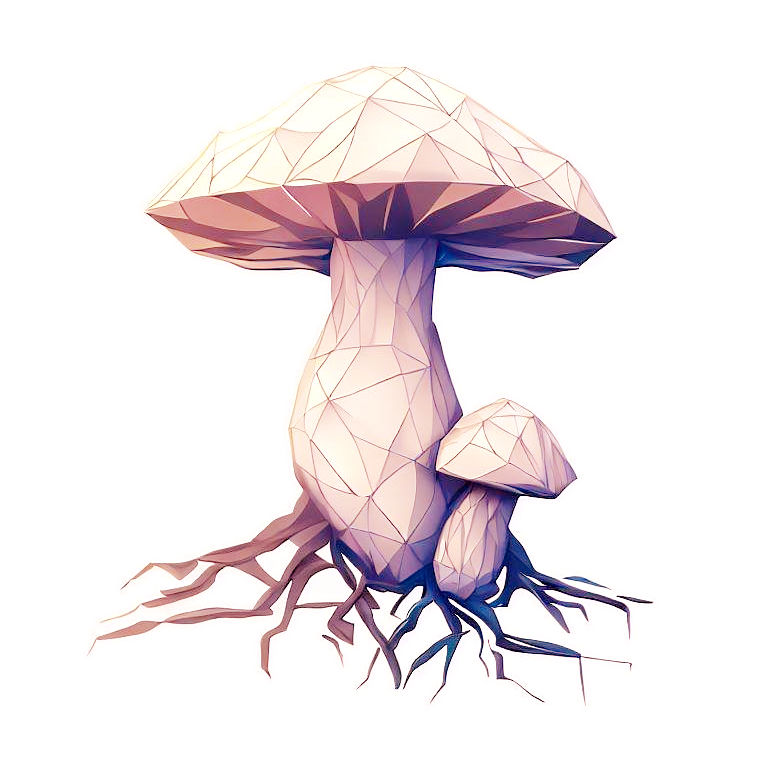
\includegraphics[height=0.15\textwidth]{solidipes.jpg}};
\node[anchor=south west, inner sep=0] (zenodo) at (-9,-1.1) {
\includegraphics[height=0.15\textwidth]{Zenodo-gradient-square.png}};

\draw[arrows = {-Stealth[inset=0pt, length=10pt, angle'=90]}, line width=4mm, color=light_purple] ($(dtool.north west) + (0.075\textwidth, 0.01\textwidth)$) -- ($(solidipes.south west) + (0.075\textwidth, -0.01\textwidth)$);
\draw[arrows = {-Stealth[inset=0pt, length=10pt, angle'=90]}, line width=4mm, color=light_purple] ($(solidipes.north west) + (0.075\textwidth, 0.01\textwidth)$) -- ($(zenodo.south west) + (0.075\textwidth, -0.01\textwidth)$);

% Labels next to images
\node[right=10pt of dtool.east, dtool] {\fontsize{16pt}{12}\selectfont\textbf{dtool}};
\node[right=10pt of solidipes.east, solidipes] {\fontsize{16pt}{12}\selectfont\textbf{solidipes}};

% the arrow
\node [
  colorbar arrow=shading4,
  label={[color=white,rotate=-90]center:data maturity}] at (8.0,-3.0) {};

\end{tikzpicture}%
\end{document}
